% Chapter 16 -- English translation of chapters/c16.tex (French source): three kernel-checked corollaries of the universal optimality theorem in openai/math
% Figure: code/fig16.py.
\chapter[Three precise certificates]{One general guarantee, three precise certificates}
\reference{Published on 10 October 2026. \doi{10.5281/zenodo.23285631}.}

\noindent\niveau{A} for the three statements, replayed in the kernel on 26 October 2026; all of them are
\emph{conditional} on an upstream theorem produced by an AI and not reviewed by peers.

\section*{The idea in one picture}

\begin{analogie}
A manufacturer publishes a general warranty: ``every appliance in family X is covered''. For your own model you
still need three checks: that your appliance really belongs to family X; that the warranty does not rest on an
infinite sum, which would make it meaningless; and that it also holds if you use the appliance in a larger or
smaller room. This chapter tells the story of signing those three certificates.

\emph{Where the picture stops:} a warranty binds whoever signs it; here, the ``general warranty'' is a theorem
written by an AI, which nobody has yet reviewed, and our certificates are worth only as much as its statement.
\end{analogie}

\section*{What was done}

On 23 September 2026, the public repository openai/math delivered a proof, written by an AI and checkable by the Lean
proof software, of a fact about arrangements of points in the plane. Picture particles that repel one another, one
per unit of area (this is called ``density~1''). Among \emph{all} the ways of placing them, not just regular
lattices, the triangular lattice (the honeycomb cells of a beehive) has the smallest total energy, for a whole
family of repulsions called ``completely monotone''. That is our general warranty.

Three consequences were drawn out and checked in Lean:
\begin{itemize}
\item \textbf{D1}: inverse-power repulsions, $1/r^s$ for every $s>0$, do belong to the family. The triangular
  lattice therefore minimises their energy.
\item \textbf{D1b}: for $s>2$, the energy of the lattice is a finite number. Without this, D1 would only say
  ``infinity is smaller than infinity''.
\item \textbf{D2}: the result holds at every density, provided the lattice is stretched in proportion.
\end{itemize}

\paragraph{An example to follow with a pencil.} Take $s=4$ and count only the near neighbours, at distance at most
$1.5$. In the triangular lattice of density~1, the nearest neighbour is at a distance $d$ with
$d^2=2/\sqrt3\approx1.155$, and there are six of them. Each costs $1/d^4=3/4$: total $6\times3/4=4.5$. In the
square lattice of the same density, four neighbours at distance~1 cost $4$, and four on the diagonals, at distance
$\sqrt2$, cost $4\times1/4=1$: total $5$. The triangular lattice is already lower. Summing over all the points, one
finds $5.783$ against $6.027$.

The trap that D2 avoids can also be computed by hand. Spread all the points of the triangular lattice apart by a
factor~2: the density falls to $1/4$ and every distance doubles, so every term $1/r^4$ is divided by $16$. The
energy becomes $5.783/16\approx0.361$. The naive statement ``the original lattice beats every configuration of
density~$1/4$'' is therefore false: that sparser lattice does much better. This counter-example is itself proved
in Lean.

\section*{How we made sure it is not wrong}

The four proof files compile, and the command that lists the starting assumptions (the \emph{axioms}) finds only
the three standard principles accepted by everyone. The same audit applied to the upstream theorem gives the same
list. Two traps planted on purpose, a gap (\texttt{sorry}) and an invented axiom, were flagged as they should be.
Another check confirms that the repulsion $t\mapsto t$, which grows with distance instead of decreasing, is indeed
\emph{rejected} by the definition.

Each result was then re-checked by another instance of the same AI model, which had not written the proofs (and
not by a human). It recompiled everything and redid its own audit, its own controls and its own calculations.
Verdict: ``confirmed with corrections'', corrections of wording and scope. A reviewer, also an AI, asked for further
corrections, which were applied. On 26 October, a complete replay in the Lean kernel, the small program that
checks every step, passed without error on the three modules.

For this book, the energies in figure~\ref{fig:c16} were recomputed in two ways, an exact formula and a direct sum
over the points, and recover the published values. These floating-point calculations illustrate; they prove
nothing.
No human mathematician has reviewed these statements.

\section*{What this does not say}

\begin{limite}
\begin{itemize}
\item Everything rests on the upstream theorem, produced by an AI and not reviewed by peers. Its statement was
  audited by AI agents, not by a human expert.
\item This is not new mathematics: each step is short, and the upstream manuscript already says that inverse powers
  are covered. The contribution is to have named statements, checked by machine and reusable.
\item The form of optimality used is slightly weaker than the reference definition in the literature; the
  repository says so in its limitations file.
\item The famous conjecture asking, for each repulsion, for a custom-made certificate is established neither
  upstream nor here.
\item For $0<s\le2$, D1 only says that the energy is infinite: the result is informative only for $s>2$.
  The divergence at $s=2$ is observed only numerically (\niveau{X}).
\end{itemize}
\end{limite}

\section*{Going further}

The paper, its Lean files and its checks are at \doi{10.5281/zenodo.23285631}, and the public repository
triangular-universal-optimality-lean is open to criticism. These corollaries served as building blocks for the
chapters on excitons, screened crystals and the interaction of thin layers, and for the student textbook.

\begin{figure}[t]
\centering
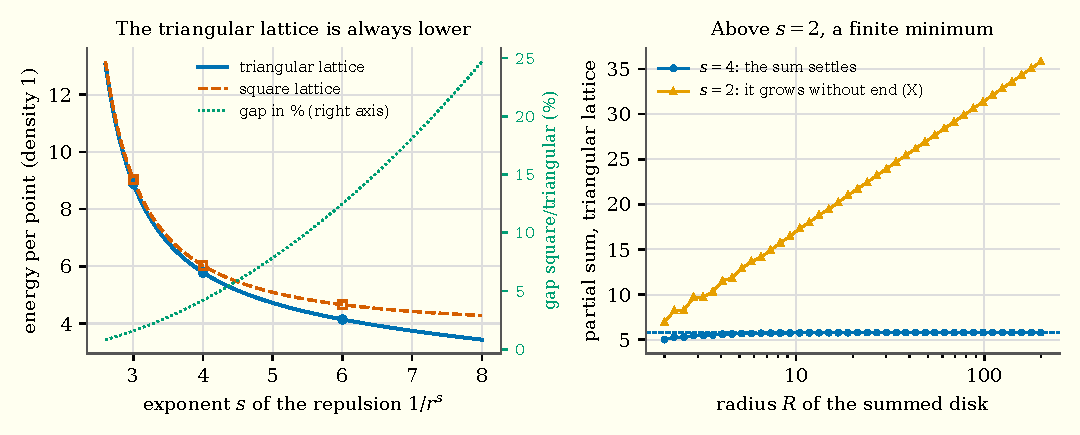
\includegraphics[width=\linewidth]{figures/c16_riesz}
\caption{Left: energy per point for a $1/r^s$ repulsion, triangular lattice against square lattice at density~1,
recomputed here (the markers are the published values). Right: partial sums over a disk of radius~$R$, which
settle for $s=4$ and grow without end for $s=2$.}
\label{fig:c16}
\end{figure}
